%
%                       This is a basic LeTeX Template
%                       for the First Year PhD literature review 
\documentclass[a4paper,12pt]{article}

\usepackage{head,fullpage}     % Add local fullpage and head macros
\usepackage{graphicx}
\usepackage{subcaption} % Add graphicx pachage with pdf flag (must use pdflatex)
\usepackage{datetime}
\usepackage{float}

\renewcommand{\dateseparator}{-}
\parindent=0pt          %  Switch off indent of paragraphs 
\parskip=5pt            %  Put 5pt between each paragraph  


\let\oldquote\quote
\let\endoldquote\endquote
\renewenvironment{quote}[2][]
  {\if\relax\detokenize{#1}\relax
     \def\quoteauthor{#2}%
   \else
     \def\quoteauthor{#2~---~#1}%
   \fi
   \oldquote}
  {\par\nobreak\smallskip\hfill(\quoteauthor)%
   \endoldquote\addvspace{\bigskipamount}}
   
   
%
%                       This section generates a title page
%                       Edit only the sections indicated to put
%                       in the project title, your name, supervisor,
%                       project length in weeks and submission date
%
\begin{document}
\begin{minipage}[b]{110mm}
        {\Huge\bf School of Physics \\and Astronomy
        \vspace*{17mm}}
\end{minipage}
\hfill
\begin{minipage}[t]{40mm}               
        \makebox[40mm]{
        
\includegraphics[width=40mm]{crest}}
\end{minipage}
\par\noindent                                           % Centre Title, and name
\vspace*{2cm}
\begin{center}
        \Large\bf Proposed Project Title\\
        \Large\bf First Year Report and Literature Review
\end{center}
\vspace*{1.5cm}
\begin{center}
        \bf Patrick Sinclair\\                 % Replace with your name
        May 2018                          % Submission Date
\end{center}
\vspace*{5mm}
%
%                       Insert your abstract HERE
%                       
\begin{abstract}
        The abstract is a short concise outline of your 
        project area, {\bf of no more than 100 words}.
\end{abstract}

\vspace*{1cm}

\vspace*{3cm}
Signature:\hspace*{8cm}Date:

\vfill
{\bf Supervisor:} Dr. Rosalind Allen                % Change to suit
\newpage
%                                               Through page and setup 
%                                               fancy headings
\setcounter{page}{1}                            % Set page number to 1
\footruleheight{1pt}
\headruleheight{1pt}
\lfoot{\small School of Physics and Astronomy}
\lhead{Literature Review}
\rhead{- \thepage}
\cfoot{}
\rfoot{Date: \ddmmyyyydate \today}
%
\tableofcontents                                % Makes Table of Contents
\pagebreak

\section{Background}

% \begin{itemize}
%  \item Antibiotic resistance - its prevalence, not understood well
%  \item overview of gradients frm martin paper - then mention a source of gradients is biofilms
%  \item Biofilms - what are they (mention polymers perhaps)
%  \item section on industrial applications - ship hulls etc
% \end{itemize}

Since their discovery in the early 1900s \cite{bioref:first-antibiotics}, antibiotics have shaped modern medicine,
and indeed modern society as a whole.  Yet despite their prevalence, with over 260,000,000 courses of antibiotics prescribed 
in the USA alone each year \cite{bioref:antibiotics-usage-USA-2011}, very little is still known about the actual 
underlying pharmacodynamics.  I.e., how these chemicals actually regulate the growth and death of bacteria.  This 
lack of understanding is becoming increasingly significant with the rising emergence of antibiotic resistance.  
There were over 58,000 deaths in newborns under the age of a year in India in 2013 due to drug-resistant 
strains of bacteria \cite{bioref:india-death-stats}, with experts predicting that the number of deaths from 
antibiotic-resistant bacteria will number in the millions by 2050 \cite{bioref:future-death-stats}.

This project aims to shed further light on how the application of antibiotics causes bacterial populations
to evolve and proliferate over time.  In particular, in the cases of when the applied antibiotic concentration has
the form of a gradient.  A considerable portion of antibiotic research has been performed under ideal conditions
with constant, uniform antibiotic concentration \cite{bioref:Grasso-constant-antibtioic-concn}, however it has only 
recently been proposed that the effects of spatial heterogeneity may be a major factor in the emergence of resistance 
and the efficacy of drugs \cite{bioref:Zhang-effects-of-antibio-grad}.  While these concentration gradients can simply arise 
due to scenarios such as diffusion throughout body tissue \cite{bioref:tissue-antibio-grads}, the scenario which is most pertinent
to this project is that of antibiotic concentration throughout biofilms.

Biofilms arise when microbial organisms adhere irreversibly to a surface and then begin to secrete various polymers which further aid
in surface and inter-microbial attachment \cite{bioref:biofilm-formation} and creates a ``slimey'' surface.  These structures are 
particularly problematic as it is difficult to achieve sufficient drug penetration to adequately curtail microbial growth, which leads to an
increase in the persistence of infections \cite{biofilms:Costerton-biofilms-persistent}.

The ability to inhibit and even prevent biofilm growth and formation has not only a multitude of medical applications, but industrial as well.
In the shipping industry it's estimated that around 10\%, up to even 45\%, of all fuel consumption of large shipping vessels arises from overcoming the 
hydrodynamic drag caused by biofilm formation on ship hulls below the water level \cite{bioref:biofilm-fuel-consumption}.  This not only has
economic influences, but also major environmental implications.  When compared to other nations, the shipping industry is the 7th largest 
producer of CO$_2$ on the planet \cite{bioref:shipping-CO2-nation}.  Therefore, research into how these marine biofilms form and develop is 
incredibly important.

Recently, several physical methods of reducing marine biofouling have been developed, which range from physical coatings that inhibit microbial
attachment due to their topography \cite{bioref:non-toxic-antifouling-strat} to usage of ultraviolet radiation \cite{bioref:UV-biofilm-repellent}.
However, the most widespread technique is that of anti-microbial paints which are applied to the boat hulls and then leach various antimicrobial
compounds over time which inhibit biofouling \cite{bioref:antimicro-paint-desc}.  It is this latter method which is of relevant interest to this project
due to its analogous nature of applying antibiotics to bacterial biofilms.

This project will involve creating simulations of a range of scenarios where bacterial populations experience antibiotic gradients, and will
investigate how these populations develop over time.  Including but not limited to; the effects of bacterial evolution, differing types of growth-rate dependent
antibiotics and populations with heterogeneous species and resistance distributions.




% Outline\cite{bioref:KUMAR19989} the background of your subject area including the key initial
% References \cite{jr:ashkin} and reference\cite{ob:Costerton1318} textbooks \cite{ob:bornwolf}. 
% Also include some of the more
% readable articles in popular science journals \cite{jr:dholakia},
% and, where appropriate, standard textbooks \cite{ob:hechtoptics}.
% 
% The exact length of this section will depend on your subject area,
% but will generally not exceed a page and will be aimed at the 
% {\it general scientific reader}. 

\section{Review of Background Bibliography}

\begin{itemize}
  \item overview of antibiotics - how they work etc
  \item Causes of antibiotic crisis
  \item growth rate dependent antibiotics, $\beta$-lactams etc
  \item how biofilms form - the bacteria change when in a biofilm, why are they difficult to get rid of 
  \item overview of biofouling, current ship hull anti-microbes
  \item difference of films and fouls
  \item brief mention of macrofouling
  \item surface colonisation
  \item opposite gradient directions for films and fouls
  \item how biocidal paint works, diffusion coefficients etc
  \item mention the differnt algorithms possible for the sims, gillespie etc - and give overview of what we used
  \item as in, mention the rates, algorithm and description of why used
 
\end{itemize}

\subsection{Antibiotic gradients}
The issue of antibiotic resistance is one of the key issues plaguing modern science as of today, and as such, the field commands a 
large volume of research dedicated to it with a wide range of methods involved, ranging from experimental to theoretical methods including both modelling and 
more in depth simulation \cite{bioref:chait-interactions, bioref:Wang-treatment-tradeoff, bioref:Torella-optimal-drug-synergy}.  While current research is 
investigating a wide variety of factors which contribute to the development of resistances, from mutational path lengths \cite{bioref:marvig-transmiss-lineage} to 
the synergistic effects of various antibiotics \cite{bioref:Liu-baicalin-synergy}, the majority of these studies, including all studies referenced
so far in this section, are performed with constant and uniform concentrations of antibiotics.

While this situation tends to be more convenient for idealised in vivo experiments, many real-world in vivo scenarios do not have these conditions.
Many naturally occurring structures, typically the ones which the drugs are intended to target, do not allow said drugs to fully permeate throughout
the region, creating drug gradients where the drug concentration can vary noticeable over space.  These gradients can arise in a variety of 
situations, from tissue \cite{bioref:minelli-peflox-penet} to bacterial biofilms \cite{bioref:Anderson2008}.

It is only in recent years that the effects of these spatial heterogeneities have been considered as a serious influencer on the evolution of resistance. 
In fact, models have been constructed which predict that drug gradients actually tend to accelerate the evolution of resistance \cite{bioref:Hermsen-source-and-sink}.
To test this hypothesis, Zhang et al. \cite{bioref:Zhang-effects-of-antibio-grad} constructed an apparatus involving an array of several interconnected microhabitats with 
an antibiotic gradient of ciprofloxacin.  This gradient ranged from no discernible antibiotic concentration at the top of the array to a concentration of 
10$\mu$g/ml at the bottom.  This concentration is around 200 times the minimum inhibitory concentration (MIC) of ciprofloxacin \cite{bioref:ciprofloxa-mic}

The array was then inoculated in the central microhabitats with around $10^6$ wild type \textit{E. coli}.  Chemotaxis due to nutrient consumption 
then drove the bacteria towards the perimeter microhabitats.  Once resistant mutants had fixed, they then spread and propagated throughout the array,
as shown in Figure \ref{fig:Zhang-gradient-apparatus}.

\begin{figure}[H]
 \centering
 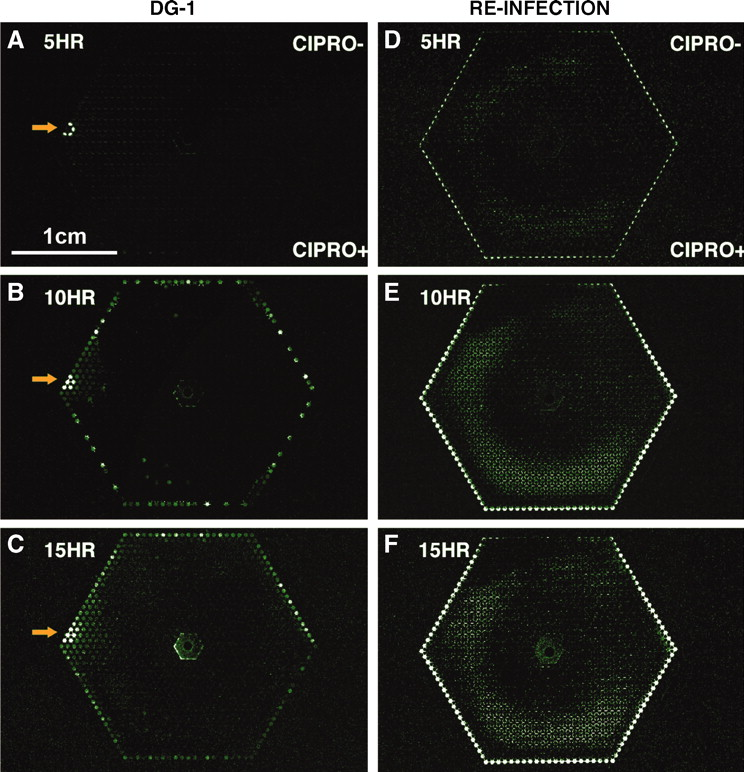
\includegraphics[width=8cm]{Zhang-microhab-gradient-cropped}
 \caption{The proliferation of the bacterial population when exposed to an antibiotic gradient.  The LHS shows the development
 of the population after the initial inoculation, and the RHS shows the development of an identical slide which was 
 inoculated with the resistant mutants. Zhang et al., 2011}
 \label{fig:Zhang-gradient-apparatus}
\end{figure}

To confirm that it was indeed the gradient which allowed for this enhanced development of resistance, Zhang et al. conducted a range of further experiments.
Firstly they eliminated the gradient by including ciprofloxacin at both ends of the array.  This uniform antibiotic concentration resulted in no growth
from the inoculated wild-type \textit{E. coli}, as can be seen in Figure \ref{fig:Zhang-gradient-growth-graph}.

\begin{figure}[H]
 \centering
 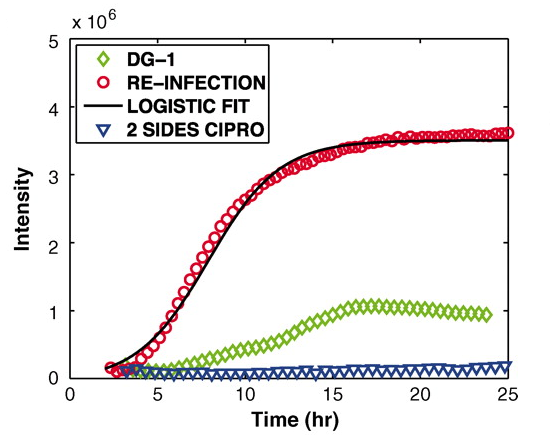
\includegraphics[width=10cm]{Zhang-microhab-gradient-growth-graph}
 \caption{The summed growth over the entire array for various scenarios.  The green diamonds are the initial experiment where the wild-type \textit{E. coli}
 were placed in the antibiotic gradient.  The red circles are the resistant mutants which were then used to re-inoculate an identically set up array.
 The blue triangles are the wild-type exposed to a uniform antibiotic concentration.  Zhang et al., 2011}
 \label{fig:Zhang-gradient-growth-graph}
\end{figure}


Zhang et al. then performed the experiment in a 96 well plate with a gradient present, but with the microhabitats now disconnected from one another, with discrete 
antibiotic concentrations in each well, ranging from low to high concentrations as in the previous array.  This also resulted in no resistance being developed,
as the growth of the bacterial colonies simply decreased as the concentration of ciprofloxacin increased, thereby implying that bacterial motility across the 
gradients is what is key to the emergence of resistance.  

To confirm the effects of motility on resistance development, Zhang et al. then used a series of agar plates with the same gradients as the microhabitat arrays,
but varied the initial population sizes.  Once they reached an initial size of $10^8$ bacteria, no motility was observed and as such growth only occurred in 
the regions of the plate where the antibiotic concentration was below the MIC, and no clear resistant mutants emerged.

Zhang et al. then proceeded to investigate what the source of the resistant mutants were, whether they were simply the descendants of already-present
mutants, or if it was indeed legitimate de novo mutation as a response to the applied antibiotic stress.  Zhang et al. reasoned that if resistance emerged due to 
preexisting, albeit rare, mutants, then either growth would have occurred above the MIC in the 96 well plate (which did not occur), or by serial dilution of the 
starting wild-type colony, they  an initial population density would eventually be reached which contained no resistant mutants, and therefore no growth would occur.


\begin{figure}[H]
 \centering
 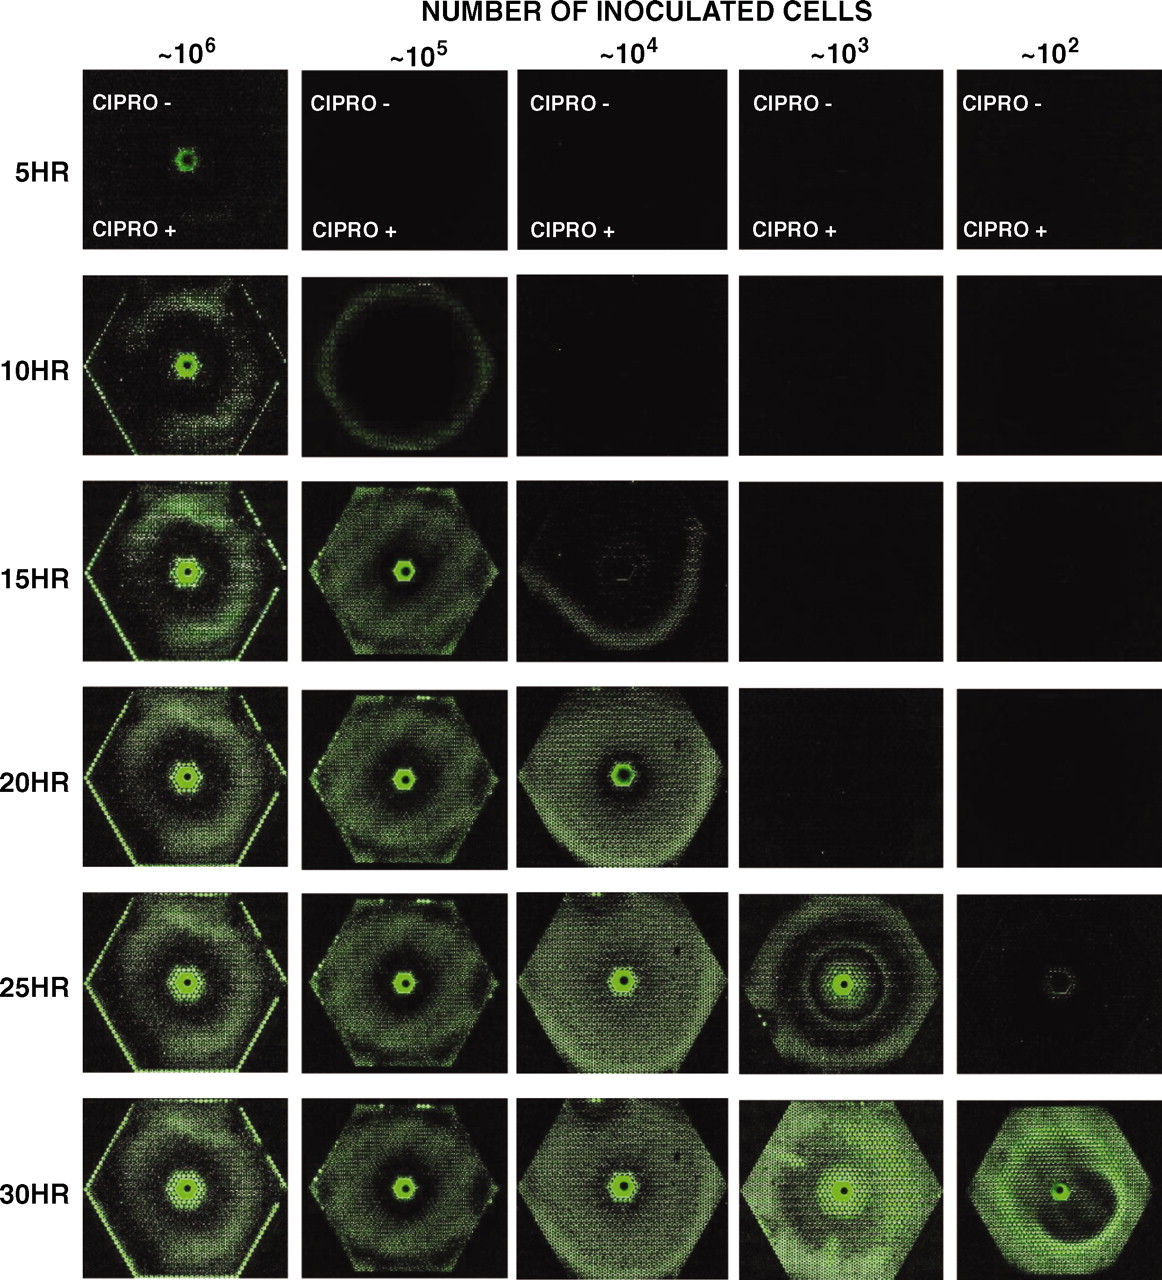
\includegraphics[height=9.6cm]{F2-large}
 \caption{Bacterial growth over time in an antibiotic gradient up to 1 $\mu$g/ml of ciprofloxacin for various initial bacterial population sizes.  
 The initial sizes range from the order of $10^6$ to as low as $10^2$.  It can be seen that even at the lowest starting densities, resistance still emerges.
 Thus supporting the argument that resistance emerges due to de novo mutation and not preexisting mutants.  Zhang et al., 2011}
 \label{fig:Zhang-gradient-inital-pop-sizes}
\end{figure}


As can be seen in Figure \ref{fig:Zhang-gradient-inital-pop-sizes}, even the most diluted populations developed resistance when exposed to the antibiotic gradient.  
These results heavily support the proposal that the source of emergent resistance is due to de novo mutations and not from preexisting mutants distributed amongst the 
wild-type.  Zhang et al. offered the following explanation as to why antibiotic gradients allow for such prevalent opportunities for resistance to emerge. 

\begin{quote}{Zhang et al., 2011}
 A spatially complex environment may lead to an enhanced rate of evolution for two reasons.  First, if a stress gradient is imposed on a connected network of 
 populations, and if a mutant acquires some resistance to the local stress, the relative fitness of the mutant is increased if it moves to join a population
 exposed to even higher stress.  Second, because there are fewer individuals in the region of higher stress, the mutant can fix more quickly in the smaller
 population.
\end{quote}

\subsection{Modelling the effects of antibiotic gradients}

As seen, there is clear experimental evidence supporting the notion that non-uniform drug distributions can accelerate the emergence of resistant organisms.  To gain 
a better understanding of whether this is always the case and also how the mutants emerge and propagate,  Greulich et al. (2012) 
\cite{bioref:PRL-drugGradients} constructed a simple computational model which investigated how a bacterial population evolved along pathways 
in genotype space when exposed to both uniform and non-uniform antibiotic concentrations.  It is this model which has also formed the basis for the other models
constructed in this project.

The model consisted of $L$ microhabitats interconnected in series with one another.  Each of which had a carrying capacity $K$ and a concentration of antibiotic present
$c_i$, where $i$ is the index of the microhabitat.  Each bacteria had a numeric genotype $m$, which they could mutate between with a probability $\mu$ 
and which had a maximum value of $M$.  This genotype described the level of resistance the bacteria had to the antibiotic.  At each step in the simulation 
each bacteria could die or move to an adjacent microhabitat at constant rates $d$ and $b$, or replicate at a rate given by 

\begin{equation}
 R_{rep} = \phi_m(c_i)(1 - \frac{N_i}{K}).
 \label{eqn:R_rep}
\end{equation}

Where $N_i$ is the total number of bacteria present in microhabitat $i$ and $\phi_m(c_i)$ is the genotype and antibiotic dependent growth rate.  
This value decreases until the MIC for that particular genotype ($\beta_m$) is reached, after which that bacteria cannot replicate.  The simulation is 
initialised by placing $K$ bacteria of genotype $m=1$ in the first microhabitat and then allowing them to proliferate throughout the system.  To illustrate the effects 
of the antibiotic gradient, the simulations were performed under two different conditions; with a uniform antibiotic concentration ($c_i = c$) and with an exponentially 
increasing antibiotic concentration ($c_i = \exp(\alpha{i}) - 1$).

\begin{figure}[H]
 \centering
 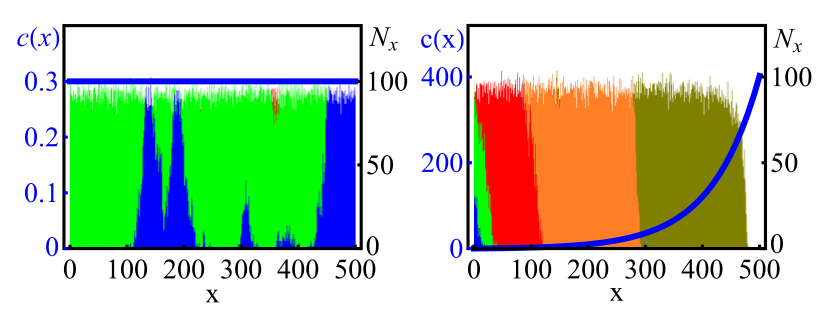
\includegraphics[height=5.6cm]{greulich-geno-distbs}
 \caption{Distributions of bacterial genotypes throughout the series of interconnected microhabitats.  The thick blue line is the concentration of antibiotic per 
 microhabitat, and the colours represent the distributions of genotypes.  $m=1$ is blue, $m=2$ green, with $m=3, 4, 5$ shown by red, orange and olive respectively.  
 For the uniform concentration, any mutations are sporadic and randomly  distributed, however the exponential gradient shows clear emergence of resistance in a 
 consistent manner.  Greulich et al., 2012.}
 \label{fig:Greulich-geno-distbs}
\end{figure}

Once again, as shown in Figure \ref{fig:Greulich-geno-distbs}, the dynamics of how evolution emerges varies greatly between the uniform and non-uniform drug distributions.  
For the uniform case, mutations arise sporadically and proliferate randomly, with the system as a whole generally evolving from one genotype to the other.  However when 
exposed to the gradient, the genotypes tend to form ``stationary fronts'', with resistant mutants emerging at the tip of the colony, then quickly spreading to fill
the remaining space until the MIC for the current advancing genotype is reached, at which point the process repeats itself.  As Figure \ref{fig:Greulich-geno-distbs} 
illustrates, where the snapshots were taken after an equal amount of time had passed, the presence of the gradient drastically reduced the time necessary for resistance 
to evolve.  To further investigate the effects of the gradients, Greulich et al. ran a series of simulations varying the overall concentration of the antibiotic for the 
uniform case, and the steepness of the gradient for the non-uniform one and recorded the time taken ($\bar{\tau}$) for a fully resistant (i.e. $m = M$) mutant to arise.


\begin{figure}[H]
 \centering
 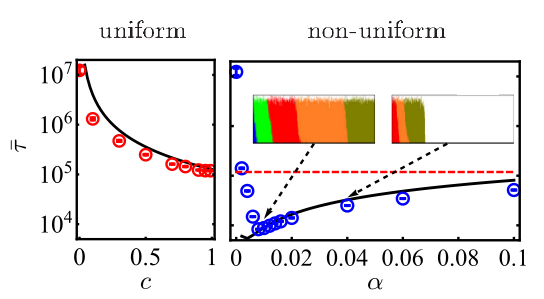
\includegraphics[height=5.8cm]{greulich-time-til-resistance}
 \caption{Time taken for a fully resistant ($m = M$) mutant to emerge for a variety of uniform drug concentrations $c$, and steepness of non-uniform drug gradient $\alpha$.  
 The red dashed line shows the minimum time taken for the uniformly concentrated system to reach resistance.  Greulich et al., 2012.}
 \label{fig:Greulich-time-til-resistance}
\end{figure}


This experiment produced an interesting result, as shown in Figure \ref{fig:Greulich-time-til-resistance}.  $\bar{\tau}$ for the uniform case followed a simple inversely 
proportional relation, which makes intuitive sense.  With a higher drug concentration present, there is also an increased pressure for resistance to emerge.  However 
for the non-uniform case, the results are somewhat more involved.  For the smallest values of $\alpha$, it's seen that the presence of the gradient actually causes $\bar{\tau}$ 
to be larger than in the uniform case, as there is much less pressure on the system for resistance to evolve.  Additionally, there seems to be an ``optimal'' value for $\alpha$, 
above which $\bar{\tau}$ begins to increase.  This is due to the fact that for the higher values of $\alpha$, the regions which the lead mutants can fill get much narrower as 
$\alpha$ increases, as seen in the snapshots included in Figure \ref{fig:Greulich-time-til-resistance}.  Thus reducing the available regions that the next generation of mutants 
can arise from.  From this it appears that the contributions of antibiotic gradients on an evolving system are even more complex than first supposed.



\subsection{Biofilms}
\begin{itemize}
 \item mention factors that affect formation, roughness etc
 \item changes undergone by bacteria in the biofilm - polymer secretions etc
 \item defense mechanisms from that paper - gradients caused by diffusions and changes in growth rates throughout the film
 \item this section will probs be the most involved
\end{itemize}

Bacteria which aggregate onto and around a surface forming a biofilm have a range of additional defences available to them which free-flowing planktonic bacterial 
colonies do not \cite{bioref:Lewis-biofilm-riddle-2001}.  These defences can afford biofilm colonies resistances to antibiotics 10-1000 times greater than their individual counterparts 
\cite{bioref:Anderson-innate-biofilm-resistances-2008}, making treatment plans an immensely more complicated affair.  These resistance mechanisms are simple to replicate in laboratory 
conditions, which heavily suggests that it is indeed the biofilm itself which possesses these qualities, rather than any external influence from the host or environment 
\cite{bioref:Stewart-biofilm-resis-mechanisms-2002}.  Biofilms can form on almost any surface where there is a consistent influx of bacteria and other microorganisms, from medical 
devices \cite{bioref:Donlan-biofilms-medical-devices-2002} to the exterior of ship hulls \cite{bioref:Chambers-modern-antifoul-coatings-2006}.  

The formation of biofilms is a complex and little-understood process.  Whilst originally thought that biofilms were formed by single organisms attaching to a surface, leading to 
the formation of micro-colonies and then 3D structures \cite{bioref:Monds-biofilm-formation-2009}, there is also now evidence that pre-existing bacterial aggregates can also 
seed the formation of biofilms \cite{bioref:hall-stooley-biofilm-clumps-2005}, the differing shape and composition of which in turn can influence the final established biofilm 
\cite{bioref:Xavier-biofilm-framework-multiD-modelling-2005}, making the developmental paths of biofilms increasingly hard to predict.

Regardless of how they come to be, biofilms have a range of features which distinguish them from a simple gathering of bacteria. One such key trait that marks them apart is that of the 
inter-cellular matrix.  When bacteria aggregate into a biofilm, they secrete a variety of macromolecules such as exopolysaccharides, DNA and protein fragments 
\cite{bioref:Whitechurch-biomatrix-components-2002}, which allows the bacteria to adhere to both surfaces and one another.

write about majority innate stuff, then diffusion and gene alteration. then do differing growth rates and that picture martin sent then done



% In this section detail the main supporting references
% and articles \cite{jr:block} for your intended area of research
% and, most importantly, your critical evaluation of their
% relevance.  Also where your subject draws from multiple 
% disciplines, do not forget to include key reference from
% each discipline, even if they are relatively old \cite{jr:dammann}. 
% 
% 
% This is the main part of your review and is the part that
% will be of use to you when preparing for your thesis. Here try
% and identify as many of the key references as possible, and enter then
% into a {\tt BibTeX} file that you will use later. Remember that recording
% the page number, titles and details of these 
% key articles {\it now} will save you hours of
% searching through {\em Web-of-Knowledge} the day before your
% submit your thesis!
% 
% This part should be written in standard scientific language, 
% aimed at the {\em experts in the field}. This is the main part of your first year report, and is 
% expected to be 10 pages in length.

\section{Progress to Date}

\begin{itemize}
 \item make several sections giving brief overview of them - PRL replication, growth dependent, multispecies 
 \item mention paper
\end{itemize}



\subsection{Greulich et al. replication}

Progress made so far in this project can be organised into several sections.  The initial few weeks of the project 
were spent replicating the results and techniques found in Greulich et al., 2012 \cite{bioref:PRL-drugGradients}.  Discussion was had
on the subject of which algorithm would be optimal for updating the system over time.  Algorithms such as Gillespie \cite{bioref:Gillespie-algorithm} 
and $\tau$-leaping \cite{bioref:tau-leap-algorithm} were proposed, but eventually a simple Monte-Carlo style selection process as detailed in the supplementary material 
of Greulich et al., was decided upon.  The purpose of this was mainly as a ``warm-up'' project.  Intended to increase fluency and familiarity in the techniques and background 
theory required for the modelling of biological systems.  The results obtained from this body of work were rough, proof-of-concept illustrations, rather than the precise 
quantitative results obtained in the actual paper.

[INSERT SOME GRAPHS AND SCREENSHOTS]


\subsection{Growth rate-dependant antibiotics}

By far the majority of the time spent on this project has been on the modelling of growth rate-dependant antibiotics, based on the 2015 paper by Greulich et al. 
\cite{bioref:Greulich-growthDependentAntibiotics}.  In this paper, Greulich et al. proposed that certain ribosome-targeting antibiotics were more effective on either 
fast-growing or slow-growing bacteria depending on how the antibiotic bound to the target ribosomes.  It's been shown that the ribosome content of a cell correlates with 
the cell's growth rate \cite{bioref:Bremer-ribosome-content-2008}, with fast-growing cells dedicating more of their resources to ribosome production than their slow-growing 
counterparts \cite{bioref:Scott-ribosome-content-2010}.  For example, the antibiotic tetracycline binds reversibly to the bacteria's ribosomes and is more effective when the 
bacteria are fast-growing.  In contrast, streptomycin binds irreversibly with the bacterial ribosomes and is more suited for bacteria which are growing slowly.  Here we 
assume that the growth rate of bacteria is directly proportional to nutrient availability, with a rich nutrient supply corresponding to a high growth rate.


The foundation of this model was heavily borrowed from the one created in the previous section, but with the key addition of nutrients, which were used to modify the 
growth rate in lieu of the carrying capacity factor from the previous model.  Two simple functional forms for the MICs of fast-growing bacteria targeting antibiotics (FGBTA)
and slow-growing bacteria targeting antibiotics (SGBTA) were constructed as follows: for the fast-growth targeting antibiotics; 

\begin{equation}
 \beta =  10 - 9\frac{\mu(S)}{\mu_{\max}}
 \label{eqn:fast-growth-beta}
\end{equation}

and for the slow-growth targeting antibiotics;

\begin{equation}
 \beta = 1 + 9\frac{\mu(S)}{\mu_{\max}}.
 \label{eqn:slow-growth-beta}
\end{equation}


Here 

\begin{equation}
 \mu(S) = \frac{S}{K' + S}
\end{equation}

where $K'$ is a constant which represents the nutrient concentration at which bacterial growth is half-maximal, the value used here is for that of \textit{E. coli} 
growing in glucose, and $S$ is a measure of the nutrients present.  Each replication by a bacteria consumes nutrients, altering the MIC in the microhabitat, 
which in turn alters the growth rate.  As $\mu_{\max}$ is a constant representing the maximum concentration of nutrients in each microhabitat, the ratio $\frac{\mu(S)}{\mu_{\max}}$ 
will decrease over time with each successful replication.  Therefore for the bacteria exposed to the fast-growth targeting antibiotics, the tip of the advancing population will be 
more inhibited than the slow-growing bulk towards the rear of the colony, and vice versa for the slow-growth targeting antibiotics.

A variety of experiments were conducted using this model, ranging from the effects of the differing types of antibiotic growth on overall population sizes, to their impact 
on spatial proliferation and how the growth rates decreased over time.  Additionally, as a form of ``control'' group, a series of experiments were also performed utilising 
growth-independent bacteria targeting antibiotics (GIBTA) whose MIC didn't vary with $S$ or $c$, but rather remained constant at all times.



\begin{figure}[H]
 \centering
 \begin{subfigure}[h]{0.49\textwidth}
 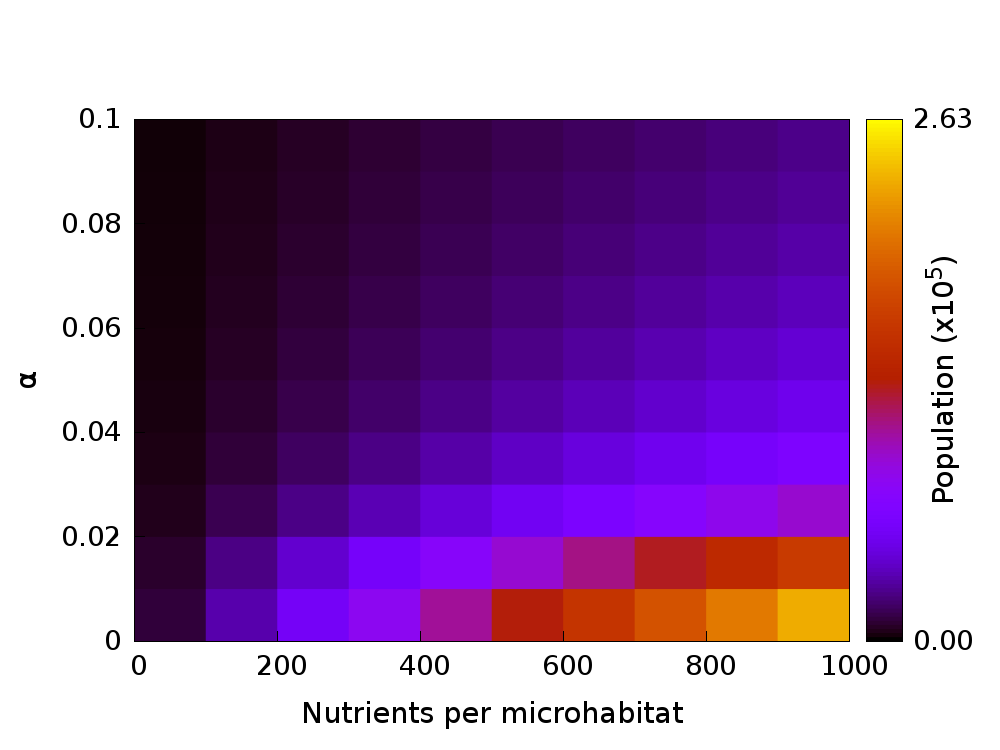
\includegraphics[width=\textwidth]{simple-slowGrowers-S_Vs_Alpha-contours}
  \caption{SGBTA}
  \label{subfig:SGBTA-alphagrad-contours}
  \end{subfigure}
  \begin{subfigure}[h]{0.49\textwidth}
  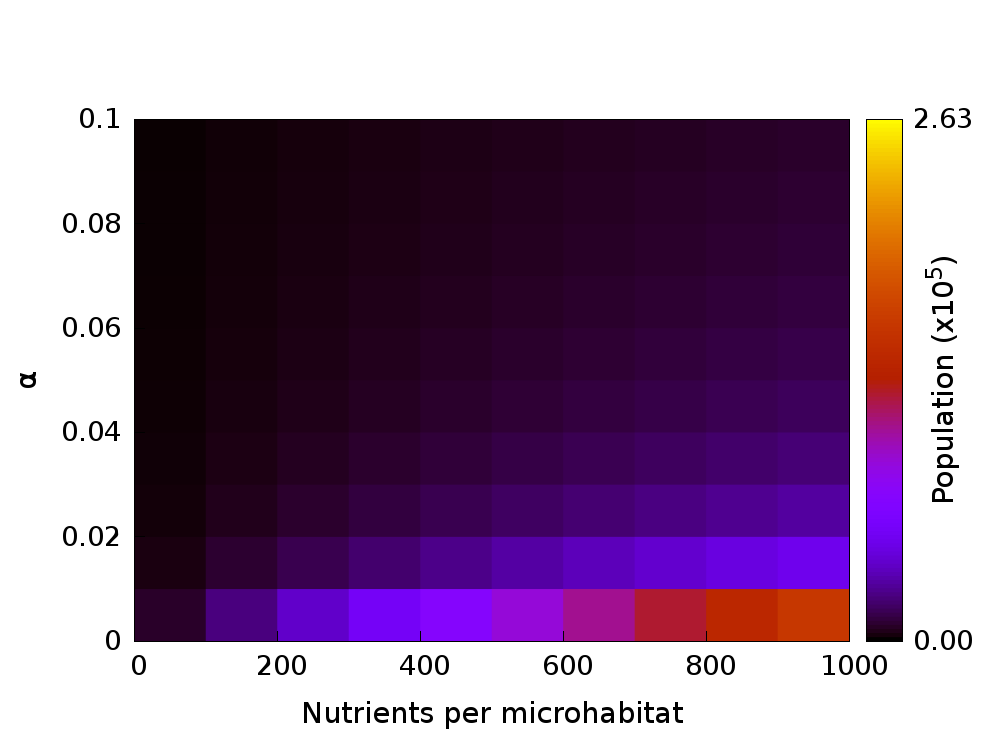
\includegraphics[width=\textwidth]{simple-fastGrowers-S_Vs_Alpha-contours}
  \caption{FGBTA}
  \label{subfig:FGBTA-alphagrad-contours}
 \end{subfigure}
\caption{Overall sizes of bacterial populations after 1000 time units have passed, for a variety of antibiotic gradients and initial nutrient concentrations.  
From this it can be seen that the SGBTA are less effective at inhibiting overall bacterial growth.}
\label{fig:alpha-popsize-contours}
\end{figure}


\begin{figure}[H]
 \centering
 \begin{subfigure}[h]{0.49\textwidth}
 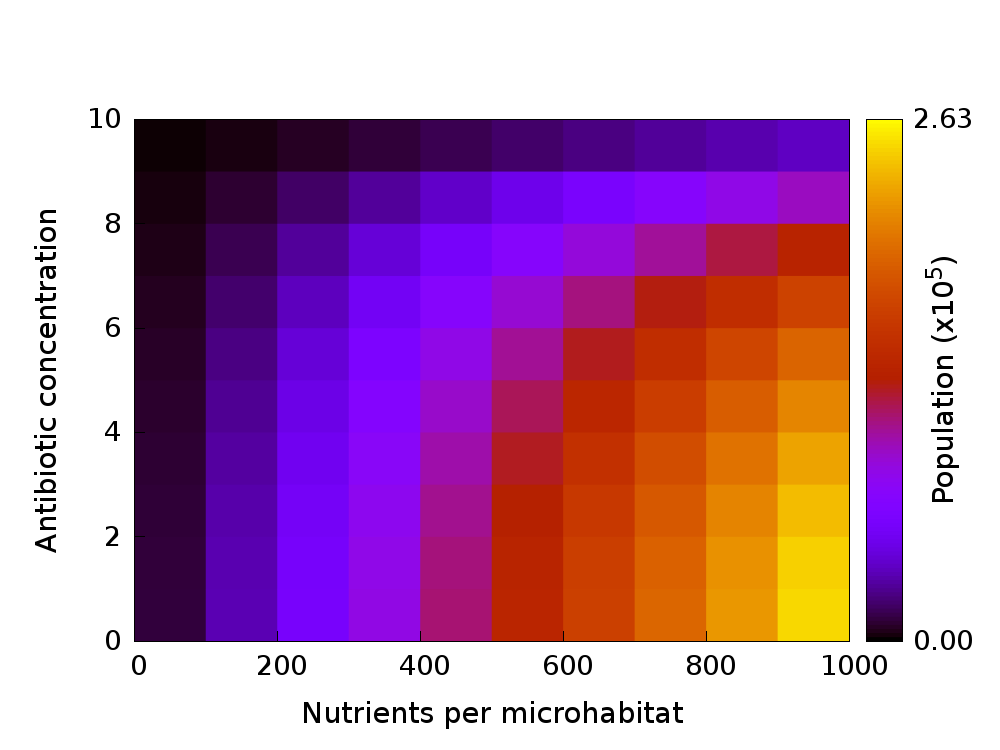
\includegraphics[width=\textwidth]{simple-slowGrowers-S_Vs_C-contours}
  \caption{SGBTA}
  \label{subfig:SGBTA-const_C-contours}
  \end{subfigure}
  \begin{subfigure}[h]{0.49\textwidth}
  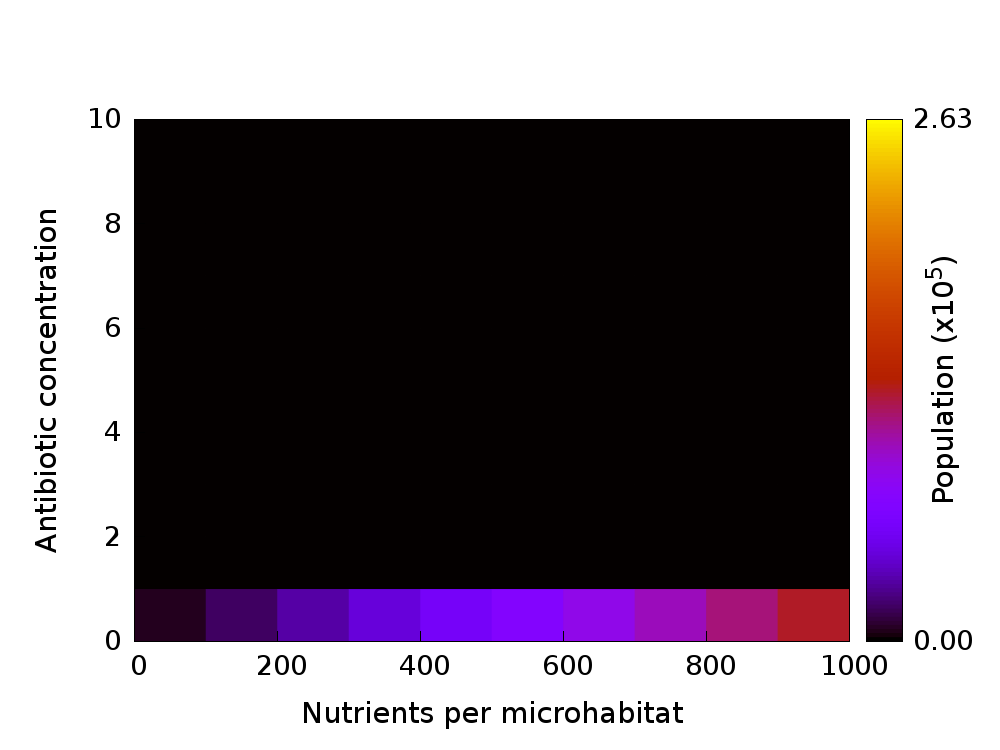
\includegraphics[width=\textwidth]{simple-fastGrowers-S_Vs_C-contours}
  \caption{FGBTA}
  \label{subfig:FGBTA-const_C-contours}
 \end{subfigure}
\caption{Overall sizes of bacterial populations after 1000 time units have passed, for a variety of uniform antibiotic and initial nutrient concentrations.  
From this it can be seen that the SGBTA are less effective at inhibiting overall bacterial growth, however the impact of a uniform antibiotic concentration has opposing effects 
for SGBTA and FGBTA.  The presence of a gradient causes the SGBTA to be more effective inhibitor, while the reverse is true for the FGBTA.}
\label{fig:const_C-popsize-contours}
\end{figure}

Some examples of the results that these experiments yielded are shown in Figures \ref{fig:alpha-popsize-contours}, \ref{fig:const_C-popsize-contours} and \ref{fig:alpha-spatdistbs}.  
Figure \ref{fig:alpha-popsize-contours} shows the total growth achieved by the bacteria for various initial nutrient concentrations and steepness of antibiotic gradients, whereas 
Figure \ref{fig:const_C-popsize-contours} utilises uniform antibiotic concentrations.  From these results two observations can be made.  Firstly, if we compare Figures 
\ref{subfig:SGBTA-alphagrad-contours} to \ref{subfig:FGBTA-alphagrad-contours} and \ref{subfig:SGBTA-const_C-contours} to \ref{subfig:FGBTA-const_C-contours}, it can be seen that 
in both cases, the SGBTA are much less effective at inhibiting the growth of the population.  However when the scenarios involving gradients are compared to those without, two 
differing features can be observed, which leads to the second observation; SGBTA are more effective inhibitors when they are applied in the form of a gradient, but the reverse is true 
for FGBTA, which are more effective in uniform concentrations.



\begin{figure}[H]
 \centering
 \begin{subfigure}[h]{0.3\textwidth}
 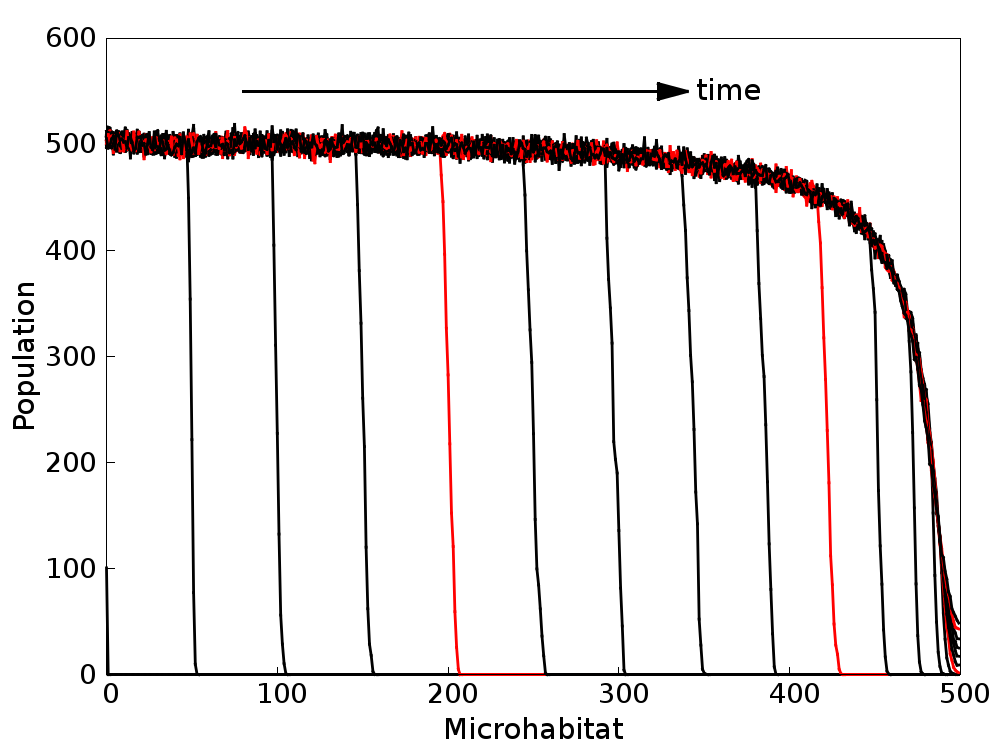
\includegraphics[width=\textwidth]{simple-slowGrowers-alpha=0_004884694070738408-spatialDistb}
  \caption{SGBTA}
  \label{subfig:SGBTA-spatdistb-spef_alpha}
  \end{subfigure}
  \begin{subfigure}[h]{0.3\textwidth}
   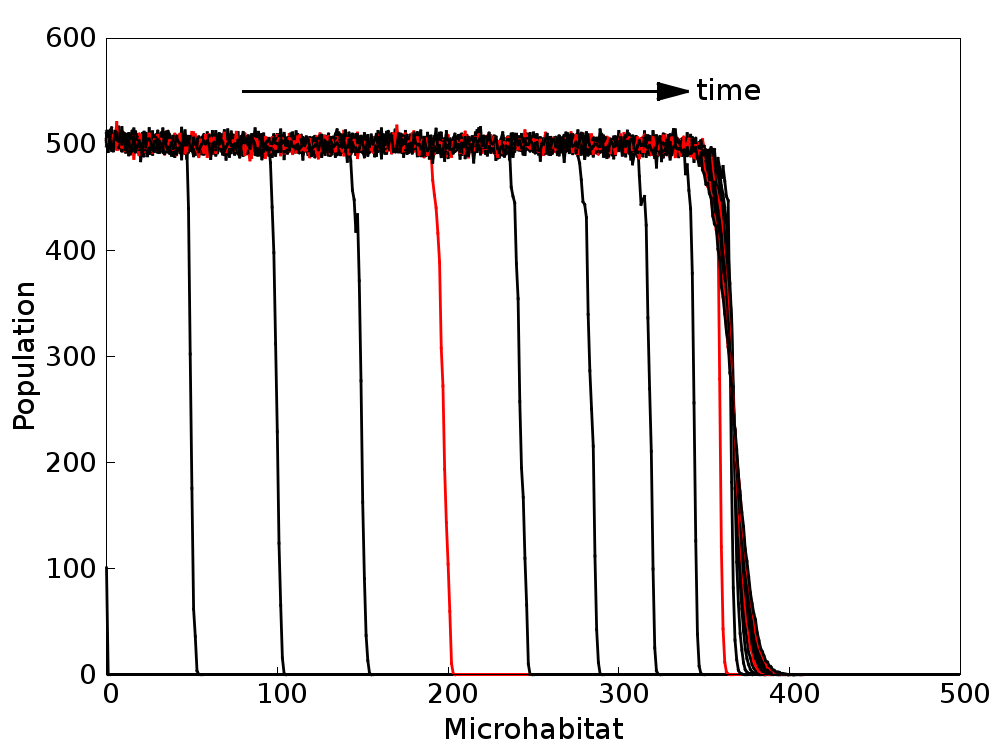
\includegraphics[width=\textwidth]{simple-flatGrowers-alpha=0_004884694070738408-spatialDistb}
   \caption{GIBTA}
   \label{subfig:GIBTA-spatdistb-spef_alpha}
  \end{subfigure}
  \begin{subfigure}[h]{0.3\textwidth}
  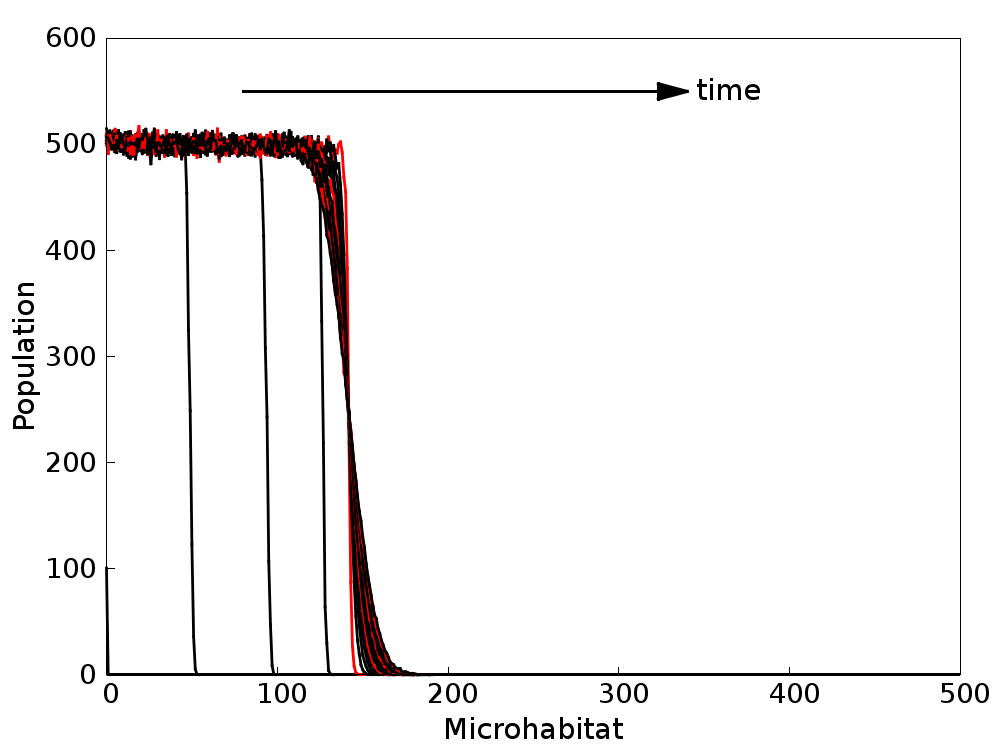
\includegraphics[width=\textwidth]{simple-fastGrowers-alpha=0_004884694070738408-spatialDistb}
  \caption{FGBTA}
  \label{subfig:FGBTA-spatdistb-spef_alpha}
 \end{subfigure}
\caption{Spatial distributions of bacterial populations exposed to SGBTA, GIBTA and FGBTA respectively.  The steepness of the antibiotic gradient has been chosen here such that 
the antibiotic concentration has a maximum of just over 10 in the final microhabitat.  Once again, the SGBTA is inferior at inhibiting bacterial growth.}
\label{fig:alpha-spatdistbs}
\end{figure}


Following on from this, simulations were run to determine how gradients of these differing antibiotic types affected the spatial distribution of the bacteria, an example of which is 
shown in Figure \ref{fig:alpha-spatdistbs}.  Here once again we can see that the SGBTA allow for the bacteria to spread much further than the FGBTA in the same timeframe, with the 
GIBTA's efficacy being somewhere inbetween the two.  Therefore showing that antibiotics which target the fast-growing tip of an advancing colony are more effective at impeding their 
progress.  

These simulations were then performed using more ``realistic'' expressions for the MICs and replication rates of relevant bacteria, from the findings in Greulich et al., 2015, which 
continue to corroborate these findings.  This component of the project has now deemed to have been completed and is currently in the process of being written up into a paper intended 
for publication.


\subsection{Multispecies models}

While many experimental investigations in laboratory conditions utilise biofilms containing only one species of bacteria, in nature the vast majority of biofilms are actually composed 
of a wide variety of species, which have differing physical properties and typically are in competition with one another \cite{bioref:Elias-biofilm-multispecies-2012}.  Motivated by 
our discussion with AkzoNobel, where they highlighted the importance of understanding how these multispecies biofilms behave in order to better design the combinations of 
anti-microbials they include in their anti-fouling paints.

To this end, work has now begun on creating a model which contains a variety of species of bacteria, each with differing resistances to the applied antibiotic.  This design is 
currently in its infancy, and is little more than a toy at the moment.  However there are plans to incorporate real lab data supplied by AkzoNobel to allow the model to utilise 
growth curves and other relevant features of observed microorganisms from real-world environments, rather than the simple numeric approximations the model currently has in place.  
Additionally discussions have been had about how best to incorporate another external source of bacteria to the system, representing the influx of microorganisms which one would 
experience in the wild.

\begin{figure}[H]
 \centering
 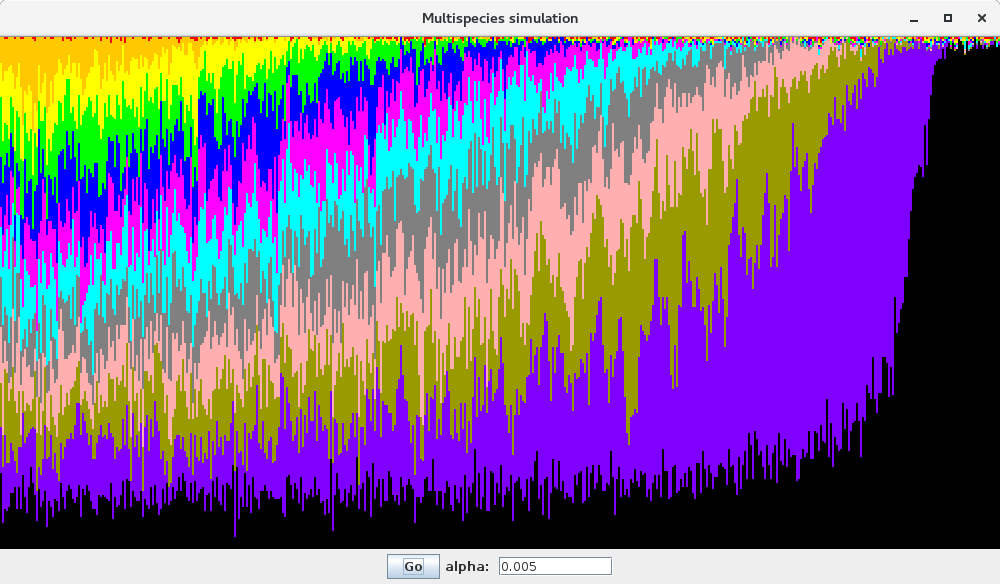
\includegraphics[height=5.8cm]{multispecies-snapshot}
 \caption{Snapshot of the GUI for the current multispecies model.  The most resistant species are shown at the bottom of the picture, with the resistances decreasing towards the top.  
 The system is exposed to an antibiotic gradient which is at its lowest on the left of the system, and increases exponentially towards the right.}
 \label{fig:Greulich-time-til-resistance}
\end{figure}



\section{Proposal}

Over the next year, the first step will be to complete writing the paper on the growth-rate dependent antibiotic model.  This should not take longer than a few weeks, as all 
the results have now been collated, so a write-up and commentary, along with a discussion section is all that remains.  Along with some mainly stylistic editing.

Following on from this, work will continue on the multispecies model.  The current version is a simplistic toy model, similar to the one in the 
Greulich paper \cite{bioref:Greulich-growthDependentAntibiotics}.  Ideally our industrial partners AkzoNobel will provide us with some more realistic parameters for factors such as 
growth and death rates for a variety of microorganisms, and their susceptibility to various biocides.  When incorporated into the current model, this should provide us with some more 
accurate, if still overly simplified, results for how a system with multiple species compete with each other over time.  Additionally, the current models only consider freely 
moving, independent bacteria.  But as seen in the previous literature, there is a vast difference between the behaviour of these  planktonic bacteria and those which have 
aggregated to form a biofilm.  As such, it seems that the next logical step is to incorporate the formation and subsequent property-altering qualities of biofilms.  I estimate 
that at least, but no more than a few months will be spent working on this model.

While these additions should certainly yield some interesting results, there is only so far that these simplistic models can take us in providing a clear picture of the mechanics 
involved in how biofilms respond to the application of antibiotics.  Therefore the plan at present is to move on from this 1D ``lattice'' model and begin work on a more 
intricate continuum model.  This model would allow us to incorporate key features of biofilms and the environment which surrounds them, such as surface roughness and flow around 
the biofilm.  These models should allow us to perform research on both the medical and industrial scenarios where biofilms form, by varying the side of the biofilm that the 
drug gradient arises from, and discerning whether these two situations create differing outcomes.  I predict that this will consume the majority of the second year of my PhD.



\begin{figure}[H]
 \centering
 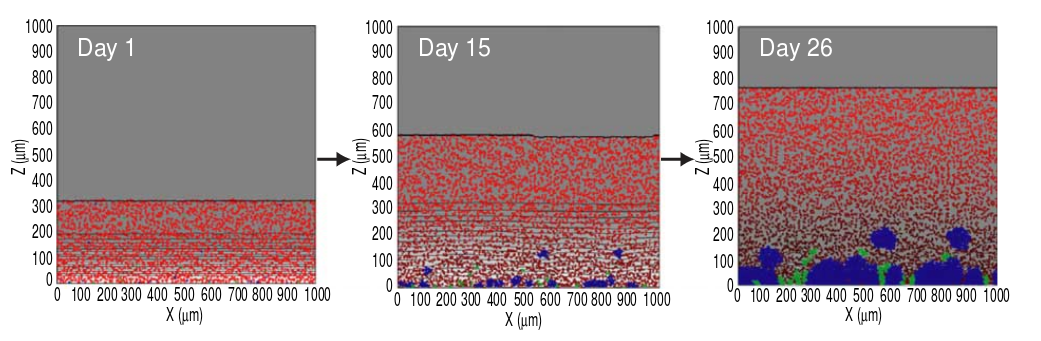
\includegraphics[width=16.4cm]{Matsumoto-biofilm-simulation}
 \caption{Screenshot taken from the paper by Matsumoto at al., 2007 \cite{bioref:Matsumoto-sim-snapshot-2007} which contained several differing species of bacteria whose growth rates 
 varied depending on the atmospheric composition of the biofilm.  This is included for illustrative purposes as an idea of what the simulations constructed in the later 
 stages of this PhD project might resemble.}
 \label{fig:Greulich-time-til-resistance}
\end{figure}

In conjunction with AkzoNobel, some wet work will be undertaken at their laboratory in Newcastle.  This would entail cultivating biofilms on various surfaces akin to industrial 
ship hulls and exposing them to a variety of biocidal paints and then examining the composition of the established biofilm to compare the model with reality.  There might also 
be opportunity to undertake part of the metagenomic analysis of these cultivated biofilms.  This aspect of the project is intended as more of an interesting aside, rather than 
as a basis of the overall PhD project.  It should only require a month or so of involvement, and will likely be performed alongside my other commitments. 

% In this section, detail, as far as you are currently able, 
% your research plan for the second and third years of your PhD, 
% drawing from the key references \cite{jr:block} that you have highlighted in your review section. 
% Here, try and illustrate
% your proposal, as in Figure~\ref{fig:prism} which is taken from the
% same paper as the illustration references.
% 
% 
% At this stage it is {\em not} expected that this will be a fully-developed
% research proposal, but is your chance to show what you have extracted from the
% literature and how you see your own work will fit in. This section is
% not expected to exceed 2 pages.
 
\section{Summary}

Simple models investigating the effects of antibiotic gradients have been constructed which demonstrate the relation between gradient steepness and time taken to evolve resistance, 
the differing inhibition properties of growth-rate dependent antibiotics and how colonies involving multiple species with differing levels of resistance develop over time.  An 
article is currently being written on the findings of the growth-rate dependent simulations.

The aim for the next year or so is to finish writing the article regarding the work on the growth-dependent antibiotics, then to continue with the multispecies
model and hopefully incorporate some realistic parameters contributed by AkzoNobel.  Following on from this, work will begin on the proposed
continuum model which could incorporate other factors such as surface texture and flow into the system.  This will be accompanied by some wet work at the AkzoNobel laboratory
at their Newcastle compound.  This is mainly for interest and not intended to form a sizable component of the project.  There has also been some discussion of
my involvement in AkzoNobel's metagenomic analysis of organisms gathered from their laboratory to extract information about the growth rates and biocidal susceptibility from 
microorganisms taken from biofilms attached to industrial shipping vessels.


\pagebreak
\newpage
%            Now build the reference list
\bibliographystyle{unsrt}                      % The reference style
%                This is plain and unsorted, so in the order
%                they appear in the document.


\bibliography{BiofilmReferences}       % Multiple bib files.

\end{document}

